\chapter{Theoretical background}
\label{ch:background} 
	\section{Web applications}
	%May be some more intro text''
		
	  Static HTML Web sites are loosing their popularity, because users
	  expect from modern Web sites more than just representing pictures and text.
	  Generally, users willing to have a highly responsive application with
	  different useful features, working in the Web. As a result Web applications are displacing Web
	  sites on the market.
	  
	   The difference of Web application from a Web site is the
	 ``ability of a user to affect the state of the business logic on the
	 server"[7]. In other words a user or a client makes a request to a server,
	 the server performs some actions (calculate, fetch data from database or
	 external Web-service) and sends the response back to the client, which is rendered in the browser see
	  figure \ref{fig:pic1}.
	  
	  \begin{figure}
      	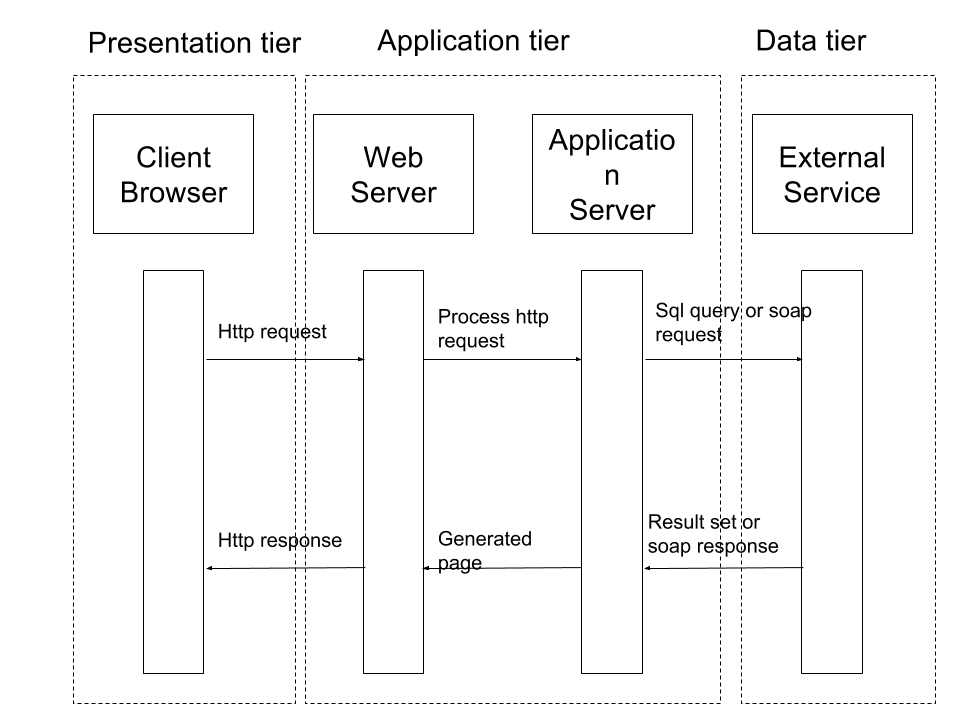
\includegraphics[width=0.75\textwidth]{client}
      	\caption{Web application structure}
      	\label{fig:pic1}
      \end{figure}
	  
    	Client-server structure helps to distribute application tasks or workloads
    	between the service providers called servers, and service requestors,
    	called clients. Client-server model helps to separate client and server logic, as
    	a result these parts can be independent and communicate via API. Client
    	server model grants several advantages:
    	\begin{itemize}
    	  \item Client and server parts can be developed separately.
    	  \item The application may have several clients.
    	  \item A client, for example a Web browser, can be already created.
    	\end{itemize}
    		
    	Client server model is closely related to a multi-tier architecture - the
    	concept where the parts of the system are divided into separate tiers. Web applications
    	 are often use three-tier architecture:
    	 \begin{itemize}
    	   \item Presentation tier is responsible for user interface generation and
    	   lightweight validation.
    	   \item Application tier (business logic tier) controls an application
    	   functionality, determines how data is created, displayed, stored and
    	   changed.
    	   \item Data tier - controls databases or other resources, provides access
    	   to the data.
    	 \end{itemize}
    	Multi-tier architecture allows any of the three tiers to be changed or
    	replaced independently, as a result developers have more freedom to use
    	external libraries and frameworks.
		
		All	applications have a lot of common features and problems which were already
		solved by developers beforehand. It is a good practise to take an already
		existing solution, than try to implement your own new one. That is why many
		modern applications are based on one or several software frameworks. In a
		rapidly changing and highly competitive business environment, choosing a right toolset is one of
		the key factors of the success.	 	
		
  \section{Vaadin}
  \label{ch:vaadin}
   ``Vaadin Framework is a Java Web application development framework that is
  designed to make creation and maintenance of high quality Web-based user interfaces easy.
   Vaadin supports two different programming models: server-side and client-side. 
   `` \cite[pr1.1]{bookVaaidn}
   \emph{Client-side} Vaadin code is executed in the Web browser as JavaScript
   code.
   \emph{Server-side} code is executed on the server as Java code on the Java
   Virtual machine(JVM).

   Client-side code is originally written in Java and then
   compiled to JavaScript using \emph{Vaadin Client Compiler}. Vaadin Client Compiler is based on Google
   Web Toolkt(GWT). The client-side code is responsible for rendering
   the user interface and send user interaction to the server. Vaadin Client
   Compiler has production and development modes. 
   
   In production mode Java  client-side code is compiled to one Javascript file. The script file in
   production mode is obfuscated, that is why reading or debugging it is nearly
   impossible. In production mode compilation should be called manually,
   after making changes to a client side Java code.
   In development mode client code is compiled at run-time, when Web page
   is reloaded. GWT links Java classes  with a compiled Javascript and gives
   an opportunity to debug code in a browser.
  
   Nowadays there are a lot of standards and recommendations for Web
   developers published by World Wide Web Consortium (W3C) or  International
   Organization for Standardization (ISO), including recommendations for
   markup languages, Document Object Models (DOM) and standards
   for JavaScript. In spite of all the standards the difference between browsers
   and versions might be significant for the developer. The differences may vary
   from supporting different Cascading Style Sheets (CSS) tags
   and HTML5 features, different event handling and simply bugs. Vaadin client Compiler and GWT provide a wide browser
   support, eliminating the difference between browsers, and helping a
   developer to concentrate on essential parts of the application, instead of
   wasting time on cross-browser support. Vaadin framework uses screenshot
   comparison see \ref{sec:screencompare} as a part of regression testing, which brings
   confidence to the developer that Vaadin components will not change their
   appearance unexpectedly. 
   
   A server-side code runs as a servlet in a Java Web server, serving HTTP
   requests.
   The ``VaadinServlet'' is normally used as the servlet class. The servlet
   receives client requests and interprets them as events for a particular user session.
   Events are associated with User Interface (UI) components and delivered to
   the event listeners defined in the application. After processing a request
   the servlet send a response back to the client and the client renders the
   changes in UI received in the response. 
   
   As mentioned before both client-side and server-side code in Vaadin is written
   in Java. This positively influences the development process in the following
   way:
   \begin{itemize}
     \item The developer does not need to know several programming languages and one
    person may be involved in the developing of both a front-end and a back-end.
    This might be an important factor for small teams and speeds up the development
    process.
   \item Vaadin brings the power of Java into the Web development. Due to
    TIOBE index \cite{tiobeIndex} Java and C are the two most popular programming
    languages since 2002. This fact allows developer to use a great amount of
    already-made solutions such as building tools Maven \cite{maven} and Ant
    \cite{ant}, testing tools like JUnit \cite{junit}, frameworks for concurrent
    applications as Akka \cite{akka} and other libraries like Yodatime \cite{yodatime}, Guava \cite{guava} for different stages of development
    process.
  \end{itemize}  		
		
\section{Testing}
		Nowadays some companies still rely on manual testing or ignore this
		important part of software development at all. Such approach has several
		sorrowful consequences:
		\begin{itemize}
			\item The developers are afraid of changing already written
			code. Because they do not have a confidence that their changes would not 
			break existing code. They stop cleaning their production code because they
			fear the changes would do more harm than good. ``Their production code begin
			to rot"
			\cite[p.123]{cleancode} 
			
			\item The effort of finding errors and	fixing them raises with the amount of
			code written, because the developers can not localize the place where the
			error is actual happening.
			\item Developing new features becomes harder, if they are based on the part
			of the system which have errors.
		
			\item Costs the whole system increases.
	 	 \end{itemize}
	 	 
	 	 To test easily the huge amount of code an automated testing is needed.	
	 	 Automated testing reduces the amount of work required to check Web applications as
	 	 well as Web sites, amplify software value, enhance reusability of test cases and improve time-to-market.
	   
		IEEE defines software testing as the process of evaluating a software
		system to verify that it satisfies specified requirements \cite{Xu1}. A set of
		requirements for a Web application includes security, performance,
		presentation, etc. We will focus on several requirements for the Web
		application which differ from desktop application. 
		
		One of the key requirements which makes testing Web applications harder than
		testing desktop application is support of different browsers and operating systems and also
		different devices. A lot of desktop applications are developed to support some
		particular operating system or different versions of the product are developed
		and maintained for different operating systems. 
		
		Web applications on the	contrary should support not only different operating systems, but also
		different browsers and devices. So, if developers team decides to support
		three operating systems (Windows, OSX, Android), three type of devices (phone,
		tablet, PC) and three browsers (Chrome, Firefox, Internet Explorer) the number
		of possible variations is already twenty seven. If you decide to support
		different version of browsers, which in some circumstances may vary a lot,
		the number of different configurations of tested machines will be close to
		one hundred. In this case manual testing is unexceptable, because it will lead
		to unwarranted expenses. 
		
		Another difference between Web and desktop applications is
		navigation on the Web page and between pages, the unexpected state change via
		the browser back button or direct Uniform Resource Locator(URL) entry in the
		browser. Some resources or parts of the application can be not
		accessible, due to connection problems or maintenance. Such unexpected
		behaviour may happen, and must be handled properly, not to crash the whole application.

    As mentioned previously one of the key factors for a successful
    development process is to pick a right toolset, this also applies to
    testing. In the chapter \ref{ch:Webtesting} we will present work done by
    other researchers and show how we can use it in creating a test framework
    for Vaadin applications.
      
\iffalse
		Web testing includes the different type of testing like:
		\begin{itemize}
		  \item functionality tests
		  \item compatibility tests
		  \item load tests
		  \item performance tests
		  \item integration tests
		\end{itemize}

		All these types of tests are equivalent important and picking a tool which
		will help to write these tests is not an easy task. 
		
		It is an advantage when	the testing tool is using same principles and similar programming language
		with other tools in the project. We think that using same programming language
		to write both tests and code is much easier for the developer. This idea is
		related to Test Driven Development(TDD), when tests are written
		before production code.
		
\fi				